\documentclass[12pt]{beamer}
\usetheme{Madrid}

\usepackage{amsmath, amsfonts}
\usepackage{hyperref}
\usepackage[super,comma,numbers]{natbib}
\renewcommand{\bibnumfmt}[1]{[#1]}
\bibliographystyle{apsrev4-1}

\title{Semi-permeable membranes as domain walls}
\author[A. Brown]{Aiyan B.}
\date{December 23, 2025}

\newcommand{\abs}[1]{\left| #1 \right|} % | |
\newcommand{\avg}[1]{\left\langle #1 \right\rangle} % < >

\begin{document}

\maketitle

\begin{frame}{Semi-permeable membranes as domain walls}
    \begin{itemize}
        \item Consider a 1d lattice of spacing $a > 0$.
        The lattice is separated by placing a semi-permeable membrane between sites $M$ and $M+1$~\cite{Das_2023},
        which can be crossed with probability $\lambda < 1$
        \item On the left of the membrane consists of a media with temporal step size $\tau_l$ and on the right a media with step size $\tau_r$ 
        -- eventually amounting to varying diffusivities
    \end{itemize}
    \begin{figure}
        \centering
        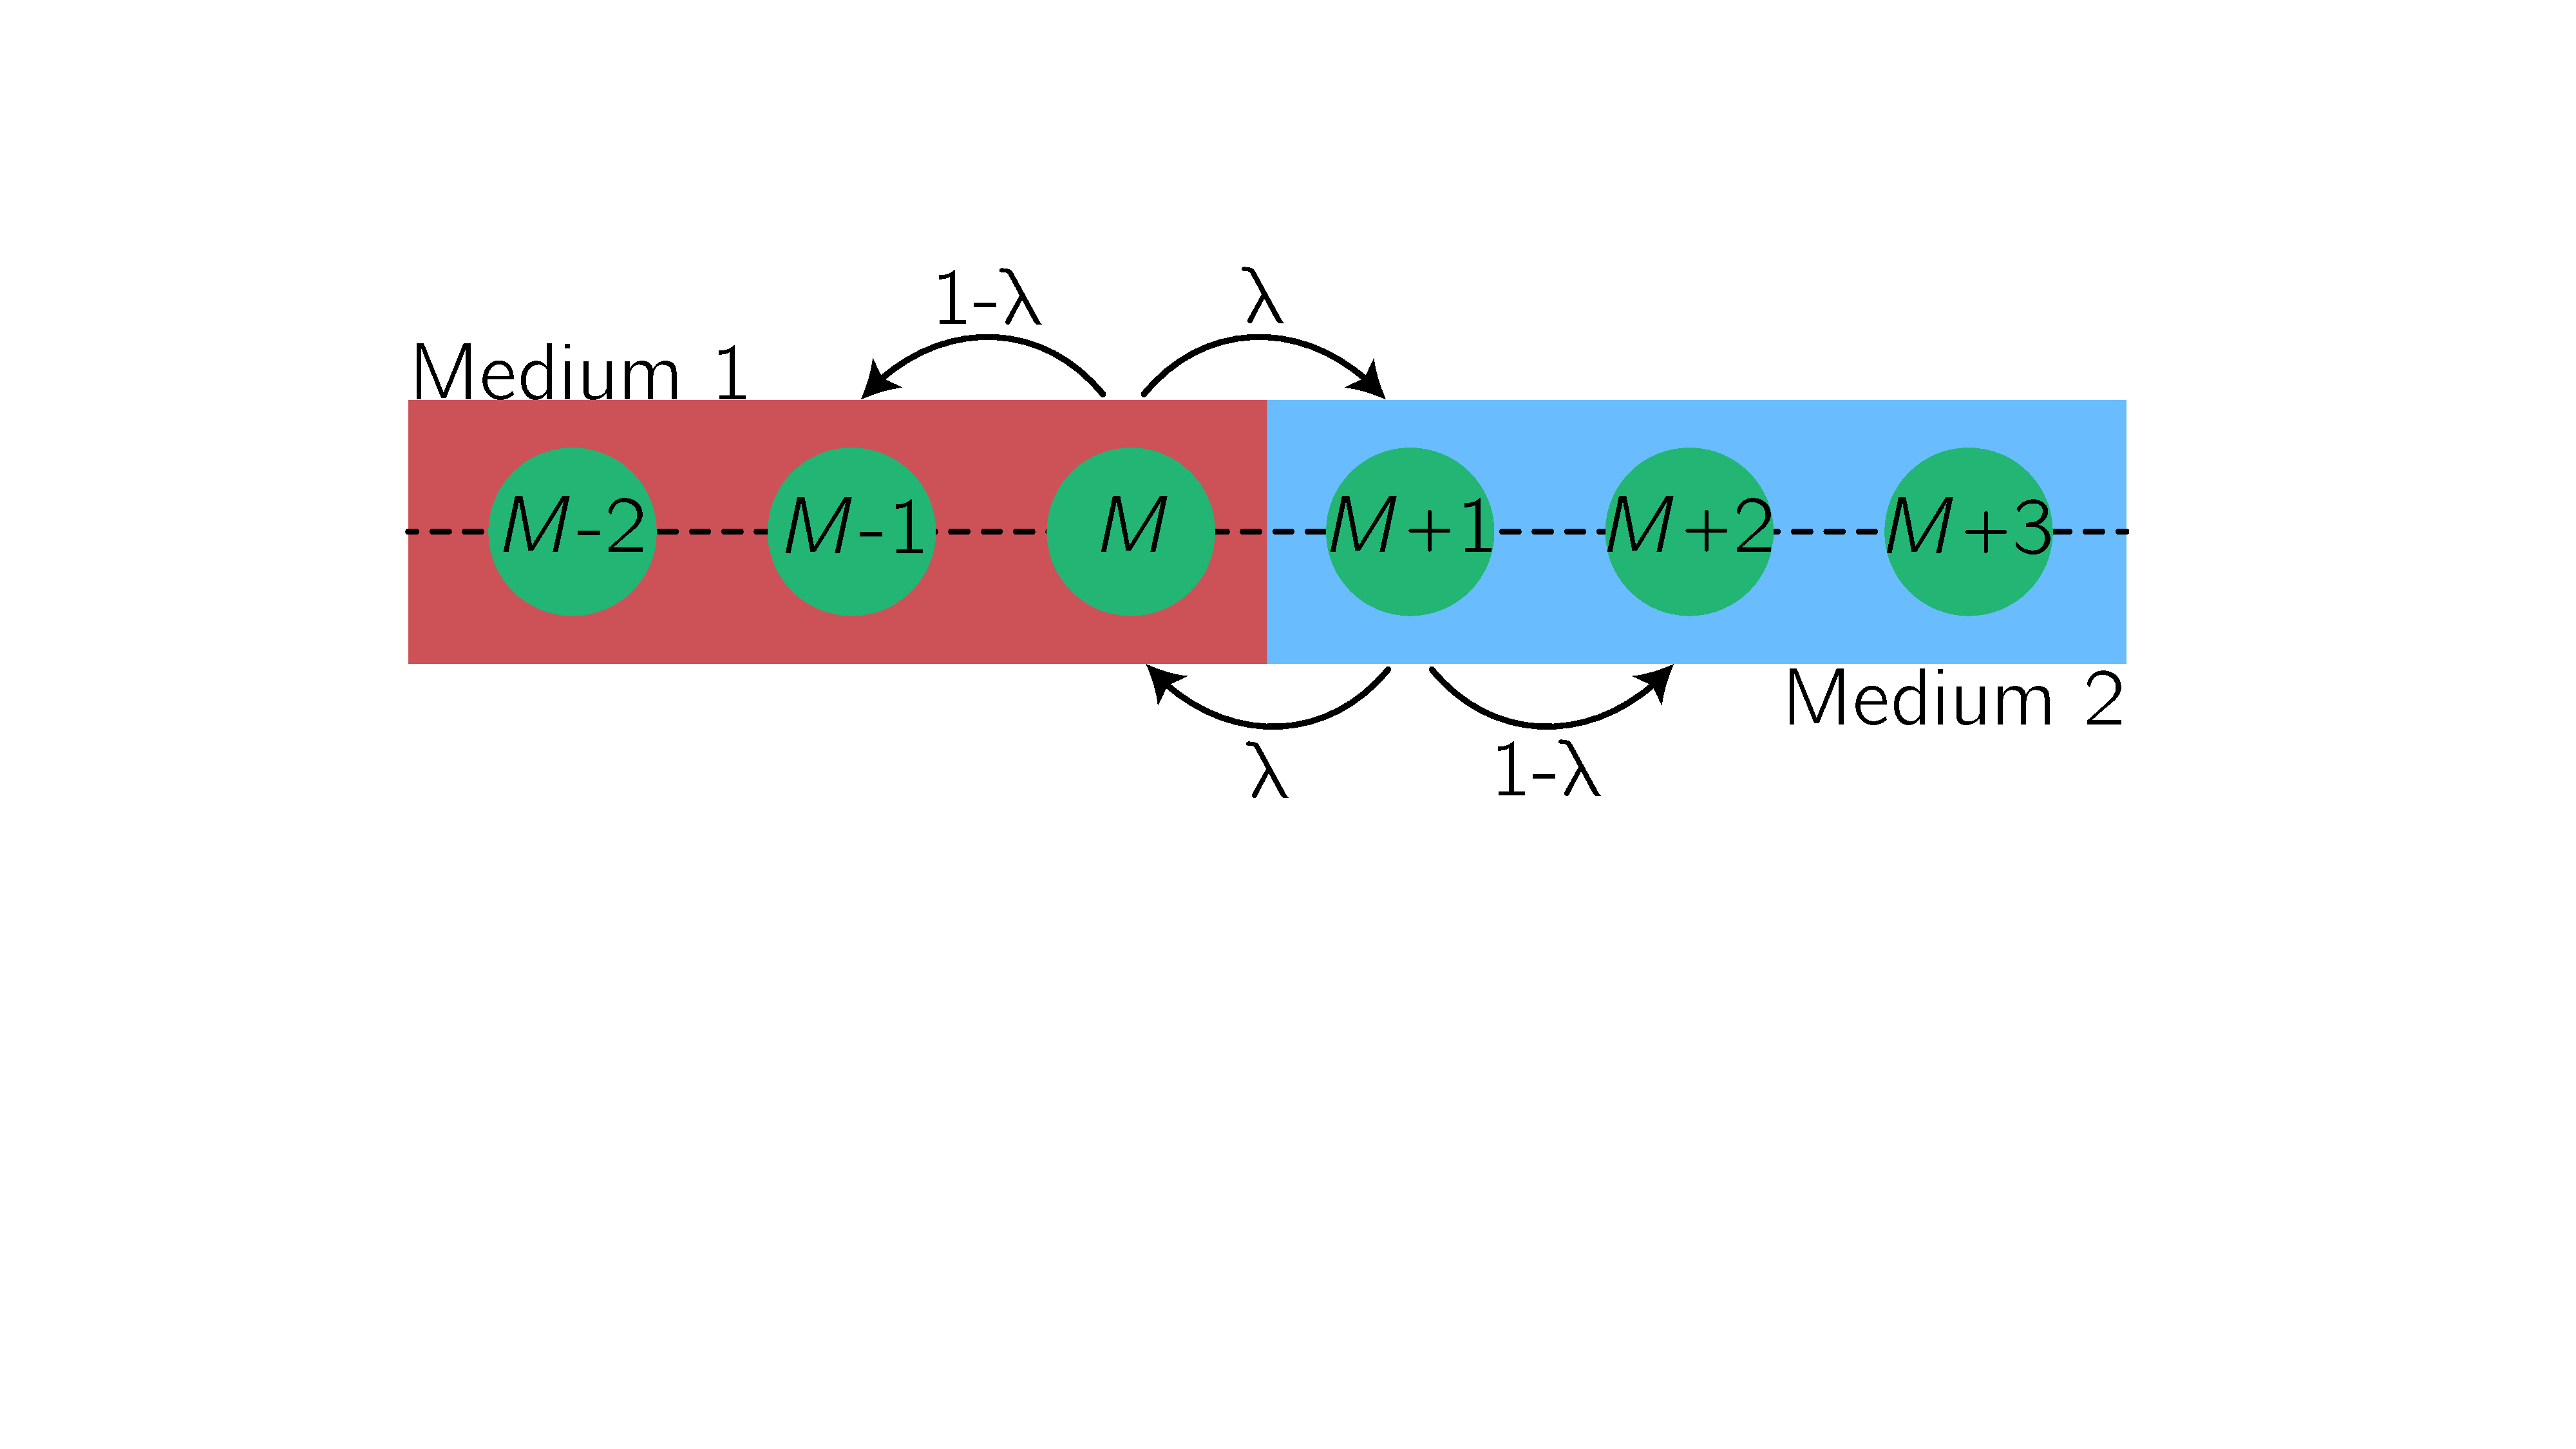
\includegraphics[width=0.9\textwidth]{figures/model.pdf}
    \end{figure}
\end{frame}

\begin{frame}{The master equation}
    \begin{itemize}
        \item Let $p_j (t)$ denote the probability of being at site $j$ at time $t$ and $\Delta = \frac{1}{2} - \lambda$.
        The (global) master equation for the system reads
    \end{itemize}
    \begin{multline} \label{eq:1}
        \frac{\partial p_j (t)}{\partial t} 
        = \left[ \frac{1}{2} p_{j + 1} + \frac{1}{2} p_{j - 1} - p_j  \right] 
        \left( \frac{1}{\tau_l} \sum_{k = - \infty}^M \delta_{j, k} + \frac{1}{\tau_r} \sum_{k = M+1}^\infty \delta_{j, k} \right) \\
        + \frac{\Delta}{\tau_l} p_M (t) \delta_{j, M-1} 
        + \frac{\Delta}{\tau_r} p_{M+1} (t) \delta_{j, M + 2} \\
        + \left( \frac{\lambda}{\tau_r} - \frac{1}{2 \tau_l} \right) p_{M+1} (t) \delta_{j,M}
        + \left( \frac{\lambda}{\tau_l} - \frac{1}{2 \tau_r} \right) p_M (t) \delta_{j,M+1}
    \end{multline}
\end{frame}

\begin{frame}{The continuum limit}
    \begin{itemize}
        \item Consider the discrete-to-continuum mapping, 
        $p_j (t) \to p (x,t)$, $M \to x_b$, $D_i = a^2 / 2 \tau_i$ and $\delta_{j,k} \to a \delta (x - y)$
        \pause
        \item Keep terms to $\mathcal{O} (a^4)$ by enforcing 
        $\kappa_i = \frac{a}{4 (2 \lambda - 1) \tau_i}$ 
        remains finite in the limit $a, \tau_l, \tau_r \to 0$,
    \end{itemize}
    \begin{multline} \label{eq:2}
        \frac{\partial p (x, t)}{\partial t} 
        = \frac{\partial}{\partial x} \left[ 
            \left( D_l \Theta(x_b-x) + D_r \Theta (x-x_b) \right) 
            \frac{\partial p (x,t)}{\partial x} 
        \right] \\
        + \left( 4 \lambda - 1 \right) \left( D_r - D_l \right) p (x_b, t) \delta' (x - x_b) \\ 
        - \frac{D_r^2}{\kappa_r} \frac{\partial p (x_b, t)}{\partial x} \delta' (x - x_b)
    \end{multline}
    \pause
    \begin{itemize}
        \item When $D_r = D_l$, diffusion becomes homogeneous across membrane 
        and we recover Kay \& Giuggioli (2022)~\cite{Kay2022}
        \item When $\lambda = 1/2$, $\kappa_r \to \infty$ and the second term remains finite
    \end{itemize}
\end{frame}

\begin{frame}{Moments}
    \begin{itemize}
        \item The mean moments of the distribution can be found by integrating with respect to $p(x,t)$.
        Using Eq.~\eqref{eq:2}, can determine the rate of change of these moments as 
        \begin{equation} \label{eq:3}
            \frac{d \avg{x^n (t)}}{dt} = \int_{- \infty}^\infty x^n \frac{\partial p (x,t)}{\partial t} \, dx
        \end{equation}
        \pause
        \item To first and second order, with $\varsigma = D_r - D_l$,
        \begin{subequations}
            \begin{equation}
                \frac{d \avg{x (t)}}{dt} 
                = 2 (1 - 2 \lambda) \varsigma p (x_b, t) 
                - \frac{D_r}{\kappa_r} J (x_b, t)
            \end{equation}
            \begin{multline}
                \frac{d \avg{x^2 (t)}}{dt} 
                = 2 \left( D_l \mathbb{P}_t (x < x_b) + D_r \mathbb{P}_t (x > x_b) \right) \\
                + 4 (1 - 2 \lambda) \varsigma x_b p (x_b, t) 
                - \frac{2 D_r x_b}{\kappa_r} J (x_b, t)
            \end{multline}
        \end{subequations}
    \end{itemize}
\end{frame}


\begin{frame}{The case of many domains}
    \begin{itemize}
        \item Our interest lies in when there is not just one domain but many.
        The generalization is straightfoward: 
        membranes are specified by the sequence of 3-tuples $\{ (x_i, \lambda_i, D_i) \}$,
        containing their position, probability of crossing, and diffusivity in the domain to their left, respectively:
    \end{itemize}
    \begin{multline}
        \frac{\partial p (x, t)}{\partial t} 
        = \frac{\partial}{\partial x} \left[ 
            \sum_i \left( D_i \Theta(x_i-x) + D_{i+1} \Theta (x-x_i) \right) 
            \frac{\partial p (x,t)}{\partial x} 
        \right] \\
        + \sum_i \left( 4 \lambda_i - 1 \right) \left( D_{i+1} - D_i \right) p (x_i, t) \delta' (x - x_i) \\ 
        + \sum_i \frac{D_{i+1}}{\kappa_{i+1}} J_i (x_i, t) \delta' (x - x_i),
    \end{multline}
    where $J_i (x, t) := - D_i \partial_x p (x,t)$ is the diffusion-driven probability current in domain $i$
\end{frame}

\begin{frame}{Specifying tuples}
    \begin{itemize}
        \item Choose to constrain each of the parameters probabilistically based on 
        physically-reasonable behaviours~\cite{PhysRevLett.112.150603}
        \pause
        \begin{enumerate}
            \item Diffusivity is bounded from below by $D_0$ such that, as $D \to D_0$, 
            the probability density scales as
            \begin{equation}
                p_D (D) \sim (D - D_0)^{\sigma - 1}, \quad \sigma > 0
            \end{equation}
            and decays exponentially for $D \gg D_0$
            \pause
            \item Given the diffusivity $D$ in a domain, impose that the 
            mean of the domain size, $r_i = x_i - x_{i-1}$, and hopping rate distributions 
            depend on the diffusivity as $D / D_0$
        \end{enumerate}
    \end{itemize}
\end{frame}


\begin{frame}{References}
    \bibliography{references}
\end{frame}

\begin{frame}{The continuum limit (details)}
    \begin{multline}
        \frac{\partial p (x, t)}{\partial t} 
        = \left[ D_l \Theta(x_b-x) + D_r \Theta (x-x_b) \right] \frac{\partial^2 p (x,t)}{\partial x^2} \\
        + a \frac{\Delta}{\tau_l} p (x_b, t) \delta (x - (x_b - a))
        + a \frac{\Delta}{\tau_r} p (x_b + a, t) \delta (x - (x_b + 2 a)) \\
        + a \left( \frac{\lambda}{\tau_r} - \frac{1}{2 \tau_l} \right) p (x_b + a, t) \delta (x - x_b) \\
        + a \left( \frac{\lambda}{\tau_l} - \frac{1}{2 \tau_r} \right) p (x_b, t) \delta (x - (x_b + a))
    \end{multline}
\end{frame}

\begin{frame}{The continuum limit (details)}
    \begin{multline}
        \frac{\partial p (x, t)}{\partial t} 
        = \left[ D_l \Theta(x_b-x) + D_r \Theta (x-x_b) \right] \frac{\partial^2 p (x,t)}{\partial x^2} \\
        + a^2 \left( 2 \lambda - \frac{1}{2} \right) p (x_b, t) \delta' (x - x_b) \left( \frac{1}{\tau_r} - \frac{1}{\tau_l} \right) \\
        + \frac{a^2}{2} \left( \frac{1}{\tau_r} - \frac{1}{\tau_l} \right) \frac{\partial p (x_b, t)}{\partial x} \delta (x - x_b) \\
        + \frac{a^3}{4} \left( \frac{1}{\tau_r} - \frac{1}{\tau_l} \right) \left[ \frac{\partial p (x_b, t)}{\partial x} \delta (x - x_b) - p (x_b, t) \delta '' (x - x_b) \right] \\
        - \frac{a^3}{\tau_r} \left( 2 \lambda - 1 \right) \frac{\partial p (x_b, t)}{\partial x} \delta' (x - x_b) + \mathcal{O} (a^4)
    \end{multline}
    \begin{itemize}
        \item The fourth term vanishes since only $\kappa_i = \frac{a}{4 (2 \lambda - 1) \tau_i}$ for $\lambda \neq 1/2$ and $D_i = a^2 / 2 \tau_i$ 
        remain finite in the $a, \tau_l, \tau_r \to 0$ limits
    \end{itemize}
\end{frame}

\end{document}